\documentclass[12pt]{report}

\usepackage[a4paper, total={17cm, 24cm}]{geometry}
\usepackage{exercise}
\usepackage{amsmath}
\usepackage{amsfonts}
\usepackage{hyperref}
\usepackage{float}
\usepackage{graphics}
\usepackage{tikz}
\usetikzlibrary{positioning}

\renewcommand{\ExerciseHeader}{\noindent\textbf{\large\ExerciseName\ %
		\ExerciseHeaderNB\ExerciseHeaderTitle
		\ExerciseHeaderOrigin\medskip}}
\setlength{\QuestionIndent}{1.5em}

\newcommand{\answerbox}[2]{\hfill\break\\
	\framebox[\linewidth]{\parbox[c][#1][c]{\dimexpr\linewidth-2\fboxsep-2\fboxrule}{#2}}
}

\renewcommand{\arraystretch}{1.2} % vertical padding for tabular environment

\begin{document}

	\hfill
	\begingroup
	\Large
	\begin{tabular}{|l|p{6cm}|}
		\hline
		First \& last name &
		% YOUR NAME HERE
		\\ \hline
		NOMA UCLouvain &
		% YOUR NOMA HERE
		\\ \hline
	\end{tabular}
	\endgroup
	\vspace{1.5cm}

	\noindent
	\begingroup
	\Large
	\textbf{LINFO2266: Advanced Algorithms for Optimization}\\\\
	Project 3: Linear Programming and Maximum Flow
	\endgroup
	\vspace{0.2cm}

	\begin{Exercise}[title={Modeling flow problems}]

		A variant of the maximum flow problem is the one with multiple sources and sinks. Fortunately, this problem can be reduced to the one with a single source and single sink and does thus not require a new algorithm.

		\Question How can you transform the following Maximum Flow Problem, with 3 sources ($s_0, s_1, s_2$) and 2 sinks ($t_0, t_1$), into a Maximum Flow Problem with 1 source and 1 sink? Answer with a clear illustration showing the reduction.

		\begin{minipage}{.45\linewidth}
				\begin{figure}[H]
				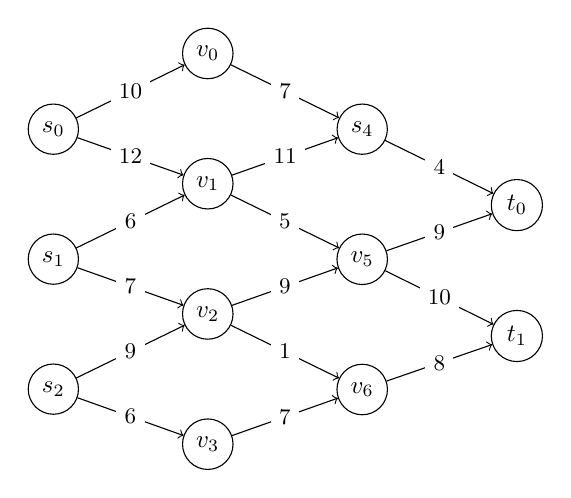
\begin{tikzpicture}[scale=0.9, every node/.style={scale=0.9}, node distance=1cm]

					\node[draw,circle] (s0) {$s_0$};
					\node[draw,circle, below=of s0] (s1){$s_1$};
					\node[draw,circle, below=of s1] (s2) {$s_2$};

					\node[draw,circle, above right=0.5cm and 1.5cm of s0] (v0) {$v_0$};
					\node[draw,circle, below=of v0] (v1){$v_1$};
					\node[draw,circle, below=of v1] (v2) {$v_2$};
					\node[draw,circle, below=of v2] (v3) {$v_3$};

					\node[draw,circle, below right=0.5cm and 1.5cm of v0] (v4) {$s_4$};
					\node[draw,circle, below=of v4] (v5){$v_5$};
					\node[draw,circle, below=of v5] (v6) {$v_6$};

					\node[draw,circle, below right=0.5cm and 1.5cm of v4] (t0) {$t_0$};
					\node[draw,circle, below=of t0] (t1){$t_1$};

					\path[->] (s0) edge node[fill=white, anchor=center, pos=0.5,font=\small\bfseries] {$10$} (v0);
					\path[->] (s0) edge node[fill=white, anchor=center, pos=0.5,font=\small\bfseries] {$12$} (v1);

					\path[->] (s1) edge node[fill=white, anchor=center, pos=0.5,font=\small\bfseries] {$6$} (v1);
					\path[->] (s1) edge node[fill=white, anchor=center, pos=0.5,font=\small\bfseries] {$7$} (v2);

					\path[->] (s2) edge node[fill=white, anchor=center, pos=0.5,font=\small\bfseries] {$9$} (v2);
					\path[->] (s2) edge node[fill=white, anchor=center, pos=0.5,font=\small\bfseries] {$6$} (v3);

					\path[->] (v0) edge node[fill=white, anchor=center, pos=0.5,font=\small\bfseries] {$7$} (v4);

					\path[->] (v1) edge node[fill=white, anchor=center, pos=0.5,font=\small\bfseries] {$11$} (v4);
					\path[->] (v1) edge node[fill=white, anchor=center, pos=0.5,font=\small\bfseries] {$5$} (v5);

					\path[->] (v2) edge node[fill=white, anchor=center, pos=0.5,font=\small\bfseries] {$9$} (v5);
					\path[->] (v2) edge node[fill=white, anchor=center, pos=0.5,font=\small\bfseries] {$1$} (v6);

					\path[->] (v3) edge node[fill=white, anchor=center, pos=0.5,font=\small\bfseries] {$7$} (v6);

					\path[->] (v4) edge node[fill=white, anchor=center, pos=0.5,font=\small\bfseries] {$4$} (t0);

					\path[->] (v5) edge node[fill=white, anchor=center, pos=0.5,font=\small\bfseries] {$9$} (t0);
					\path[->] (v5) edge node[fill=white, anchor=center, pos=0.5,font=\small\bfseries] {$10$} (t1);

					\path[->] (v6) edge node[fill=white, anchor=center, pos=0.5,font=\small\bfseries] {$8$} (t1);

				\end{tikzpicture}
			\end{figure}
		\end{minipage}
		\hfill
		\begin{minipage}{.54\linewidth}
			\answerbox{9cm}{
				% YOUR ANSWER HERE
			}
		\end{minipage}


		\Question The \texttt{FlowNetwork} with $V$ vertices and $E$ edges, can be solved with a Linear Programming formulation
		of the form $\{ \max \ c \cdot x \mid A \cdot x \leq b, x \geq 0 \}$.
		Give the dimensions (number of variables and constraints) of the matrix $A$ expressed
		using the cardinalities of $V$ and $E$.
		\answerbox{2cm}{
			% YOUR ANSWER HERE
		}


	\end{Exercise}

	\begin{Exercise}[title={Experimental comparison LP vs Dedicated Algorithm}]

		We are interested to compare experimentally the time required by the Ford-Fukerson algorithm and the linear program for solving
		the maximum flow problem. We can perform time measurement on benchmark instances and report them graphically.
		Given the 50 instances \texttt{flowXXXX\_YYYY.txt} within the \texttt{data/Flow} directory, analyze the running time of the 2 algorithms and give your observations.


		\Question Give the cactus plot of the running time to solve the instances between a \texttt{FlowMatrices} (+ the corresponding call to \texttt{LinearProgramming} to solve it) and a \texttt{FordFulkerson} solver. Your \textit{x} axis should be the maximum time allowed (in log scale) and the \textit{y} axis the cumulated number of problems solved within the maximum time. You can find one example of such a plot \href{https://jeremiasberg.files.wordpress.com/2021/10/cactus_plot_side_v4.jpg?w=346&h=205}{here}.
		\answerbox{8cm}{
			% YOUR ANSWER HERE
		}

		\Question Which solver performs best according to the cactus plot? Comment the differences you observe between the two methods, solely based on the plot.
		\answerbox{1.5cm}{
			% YOUR ANSWER HERE
		}

		\pagebreak

		\Question Give a comparison plot of the log-running time to solve the instances between a \texttt{FlowMatrices} (+ the corresponding call to \texttt{LinearProgramming} to solve it) and a \texttt{FordFulkerson} algorithm solver. Your \textit{x} axis needs to be related to the log run time \texttt{FlowMatrices} formulation and your \texttt{y} axis to the log run time the \texttt{FordFulkerson}. Draw a diagonal line $x=y$ to ease the comparison. You can find one example of such a plot \href{https://www.researchgate.net/profile/Gael-Glorian/publication/335984300/figure/fig3/AS:827659797925888@1574340881515/Picasso-vs-gc-cdcl.png}{here}
		\answerbox{8cm}{
			% YOUR ANSWER HERE
		}

		\Question Which solver performs best according to the comparison plot? Comment the differences you observe between the two methods, solely based on the plot. What is the link with the diagonal line and what does it represent?
		\answerbox{1.5cm}{
			% YOUR ANSWER HERE
		}


	\end{Exercise}


\end{document}